% !TeX spellcheck = ru_RU
%\documentclass[a4pape, 14pt]{extarticle} % расширенный класс статьи с возможностью указать 14 шрифт
%\documentclass[a4pape, 11pt]{article}
\documentclass[oneside, final, 14pt]{extarticle}
\usepackage{graphicx}  % поддержка .eps-графики
\usepackage[utf8]{inputenc} % кодировка в которой набран текст 
\usepackage[T2C]{fontenc} % поддержка кирилицы % ещё можно T1 T2B T2A T2
\usepackage[english,russian]{babel} % переносы и типографские правила для русского
\usepackage{indentfirst}  % красная строка
\usepackage{listings}  % оформление листингов программ
\usepackage{amssymb,amsfonts,amsmath,mathtext} % ядро для научной статьи
\usepackage{physics}
\usepackage{mathtools}
\usepackage{braket}
\usepackage{float} % для рисунков
\usepackage{array} % для m{2cm} в таблицах
\usepackage{blindtext} % случайный текст для заглушки

\usepackage{titlesec}
%\linespread{1.3}
%\usepackage{setspace}\onehalfspacing
%\usepackage{vmargin} отступы из книги столярова
%\setpapersize{A4}
%\setmarginsrb{2.5cm}{2cm}{1.5cm}{2cm}{0pt}{0mm}{0pt}{13mm}


%\usepackage{sectsty} % не работает с extarticle. Должно было уменьшить размер заголовков
%\sectionfont{\fontsize{14}{14}\selectfont}

\usepackage{titlesec} % https://ru.overleaf.com/learn/latex/Sections_and_chapters % пакет для изменения заголовков разделов
\titleformat{\section}
{\normalfont\fontsize{14}{14}\bfseries}{\thesection}{1em}{}

\usepackage{pdfpages} % для вставки пдф файлов

\usepackage{pgfplots} % построение графиков
% We will externalize the figures
%\usepgfplotslibrary{external}
%\tikzexternalize
%\pgfplotsset{width=15cm,compat=1.5}

%\sloppy
%\fussy

\usepackage[left=2cm, right=2cm, top=1.5cm, bottom=1.5cm]{geometry} % установка полей

\newcommand{\hup}{Принцип неопределенности Гейзенберга}
\newcommand{\qe}{Квантовая запутанность}

%\usepackage{citehack}  % https://www.opennet.ru/docs/RUS/cyr_howto/ch08s02.html
%\usepackage[bibencoding=auto,backend=biber,babel=other]{biblatex}
%\usepackage{csquotes} 


% https://ru.overleaf.com/learn/latex/Pgfplots_package  - для построения графиков
% https://ru.overleaf.com/learn/latex/Tables - построение таблиц
% https://ru.overleaf.com/learn/latex/Commands - обьявление команд
\graphicspath{{./images/}} %путь к рисункам
\frenchspacing % длина пробелов после пунктуации
\pagestyle{plain}
\selectlanguage{russian}
\bibliographystyle{gost780} % gost780 - сортировка по порядку следования, gost780s - по алфавиту кажется. gost780u не завелся

\begin{document}

\begin{titlepage}
	\centerline{
\includegraphics[width=2cm]{dstu-logo}}
	\vfill
	%\Large
	\centerline{МИНЕСТЕРСТВО НАУКИ И ВЫСШЕГО ОБРАЗОВАНИЯ}
	\centerline{РОССИЙСКОЙ ФЕДЕРАЦИИ}
	\vfill
	\centerline{\bf ФЕДЕРАЛЬНОЕ ГОСУДАРСТВЕННОЕ БЮДЖЕТНОЕ}
	\centerline{\bf ОБРАЗОВАТЕЛЬНОЕ УЧРЕЖДЕНИЕ ВЫСШЕГО ОБРАЗОВАНИЯ}
	\centerline{\bf «ДОНСКОЙ ГОСУДАРСТВЕННЫЙ ТЕХНИЧЕСКИЙ УНИВЕРСИТЕТ»}
	\centerline{\bf (ДГТУ)}
	\normalsize
	\vfill\vfill
	\centerline{Факультет «Отдел аспирантуры и докторантуры»}
	\centerline{Кафедра «Кибербезопасность информационных систем»}
	\vfill
	%\rightline{Место для подписи завкафедрой}
	\vfill
	%\Large{\centerline{\bf ПОРТФОЛИО АСПИРАНТА}}
	\centerline{План-проспект реферата по дисциплине «История и философия науки»}
%	\centerline{«История и философия науки»}
	\centerline{на тему «История и философия криптографии»}
	\vfill
	\vfill
	\vfill
	\vfill
	\vfill
	\vfill
	\vfill
	\rightline{Выполнил:}
	\rightline{аспирант 1го курса}
	\rightline{по направлению подготовки}
	\rightline{09.06.01 «Информатика и вычислительная техника»}% номер зачетной книжки: 2142748
	\rightline{Галов К.А.}
	\rightline{Проверил: д.ф.н., доцент Тазаян А.Б.} % Тазаян Араван Бабкенович
	\vfill
	\vfill
	
	\centerline{г. Ростов-на-Дону}
	\centerline{2022 г.}
	
\end{titlepage}
\setcounter{page}{2}

\section*{Введение}
%Определение криптографии. Актуальность этого раздела науки. Цель криптографии.
Криптография - наука о методах обеспечения конфиденциальности, целостности и подлинности авторства, а также невозможности отказа от авторства информации.

Изначально криптография изучала методы шифрования информации — обратимого преобразования исходного текста на основе секретного алгоритма или ключа в шифрованный текст. Традиционная криптография образует раздел симметричных криптосистем, в которых зашифрование и расшифрование проводится с использованием одного и того же секретного ключа. Помимо этого раздела современная криптография включает в себя асимметричные криптосистемы, системы электронной цифровой подписи, хеш-функции, управление ключами, получение скрытой информации, квантовую криптографию.

Криптография — одна из старейших наук, её история насчитывает несколько тысяч лет. И в 21 веке эта наука не теряет своей актуальности, решая ряд важнейших задач:
\begin{itemize}
	\item cобственно шифрование данных с целью защиты от несанкционированного доступа;
	\item проверка подлинности сообщений: получатель сообщения может проверить его источник;
	\item проверка целостности передаваемых данных: получатель может проверить, не было ли сообщение изменено или подменено в процессе пересылки;
	\item обеспечение невозможности отказа, то есть невозможности как для получателя, так и для отправителя отказаться от факта передачи;
	\item скрытие информации.
\end{itemize}

Проблемой защиты информации при ее передаче между абонентами люди занимаются на протяжении всей своей истории. Человечеством изобретено множество способов, позволяющих в той или иной мере скрыть смысл передаваемых сообщений от противника.

%\section{Идеалы и нормы научности в криптографии}
%Принципы написания научных работ по криптографии. Идеализация участников канала связи.
% обычные принципы + то, что злоумышленник ограничен только законами физики.

%Литература: \cite{phil2016nesm, scarani2004quantum}

\clearpage

\section{Периоды развития и этапы криптографии}
В качестве основного критерия периодизации криптографии возможно использовать технологические характеристики используемых методов шифрования. В данном реферате будем придерживаться такой периодизации.

Первый период (приблизительно с 3-го тысячелетия до н.э.) характеризуется господством моноалфавитных шифров (основной принцип – замена алфавита исходного текста другим алфавитом через замену букв другими буквами или символами).

Второй период (хронологические рамки – с IX века на Ближнем Востоке (Ал-Кинди) и с XV века в Европе (Леон Баттиста Альберти) – до начала XX века) ознаменовался введением в обиход полиалфавитных шифров.

Третий период (с начала и до середины XX века) характеризуется внедрением электромеханических устройств в работу шифровальщиков. При этом продолжалось использование полиалфавитных шифров.

Четвёртый период – с середины до 70-х годов XX века – период перехода к математической криптографии. В работе Клода Шеннона появляются строгие математические определения количества информации, передачи данных, энтропии, функций шифрования. Обязательным этапом создания шифра считается изучение его уязвимости к различным известным атакам – линейному и дифференциальному криптоанализу. Однако до 1975 года криптография оставалась «классической», или же, более корректно, криптографией с секретным ключом.

Современный период развития криптографии (с конца 1970-х годов по настоящее время) отличается зарождением и развитием нового направления – криптография с открытым ключом. Её появление знаменуется не только новыми техническими возможностями, но и сравнительно широким распространением криптографии для использования частными лицами (в предыдущие эпохи использование криптографии было исключительной прерогативой государства). Правовое регулирование использования криптографии частными лицами в разных странах сильно различается – от разрешения до полного запрета.

Историю криптографии условно можно также разделить на 4 этапа\cite{scarani2004quantum}.

\begin{itemize}
	\item Наивная криптография.
	\item Формальная криптография.
	\item Научная криптография.
	\item Компьютерная криптография.
\end{itemize}


Для наивной криптографии (до нач. XVI века) характерно использование любых (обычно примитивных) способов запутывания противника относительно содержания шифруемых текстов. На начальном этапе для защиты информации использовались методы кодирования и стеганографии, которые родственны, но не тождественны криптографии. Большинство из используемых шифров сводились к перестановке или моноалфавитной подстановке. Одним из первых зафиксированных примеров является шифр Цезаря, состоящий в замене каждой буквы исходного текста на другую, отстоящую от нее в алфавите на определенное число позиций. Другой шифр, полибианский квадрат, авторство которого приписывается греческому писателю Полибию, является общей моноалфавитной подстановкой, которая проводится с помощью случайно заполненной алфавитом квадратной таблицей (для греческого алфавита размер составляет 5x5). Каждая буква исходного текста заменяется на букву, стоящую в квадрате снизу от нее.

Этап формальной криптографии (кон. XV века - нач. XX века) связан с появлением формализованных и относительно стойких к ручному криптоанализу шифров. В европейских странах это произошло в эпоху Возрождения, когда развитие науки и торговли вызвало спрос на надежные способы защиты информации. Важная роль на этом этапе принадлежит Леону Батисте Альберти, итальянскому архитектору, который одним из первых предложил многоалфавитную подстановку. Данный шифр, получивший имя дипломата XVI века Блеза Вижинера [4], состоял в последовательном «сложении» букв исходного текста с ключом (процедуру можно облегчить с помощью специальной таблицы). Его работа «Трактат о шифре» считается первой научной работой по криптологии. Одной из первых печатных работ, в которой обобщены и сформулированы известные на тот момент алгоритмы шифрования является труд «Полиграфия» немецкого аббата Иоганна Трисемуса. Ему принадлежат два небольших, но важных открытия: способ заполнения полибианского квадрата (первые позиции заполняются с помощью легко запоминаемого ключевого слова, остальные - оставшимися буквами алфавита) и шифрование пар букв (биграмм). Простым, но стойким способом многоалфавитной замены (подстановки биграмм) является шифр Плейфера, который был открыт в начале XIX века Чарльзом Уитстоном. Уитстону принадлежит и важное усовершенствование - шифрование ««двойным квадратом». Шифры Плейфера и Уитстона использовались вплоть до первой мировой войны, так как с трудом поддавались ручному криптоанализу. В XIX веке голландец Керкхофф сформулировал главное требование к криптографическим системам, которое остается актуальным и поныне: секретность шифров должна быть основана на секретности ключа, но не алгоритма. Наконец, последним словом в донаучной криптографии, которое обеспечили еще более высокую криптостойкосить, а также позволило автоматизировать (в смысле механизировать) процесс шифрования стали роторные криптосистемы. Одной из первых подобных систем стала изобретенная в 1790 году Томасом Джефферсоном, будущим президентом США механическая машина. Многоалфавитная подстановка с помощью роторной машины реализуется вариацией взаимного положения вращающихся роторов, каждый из которых осуществляет «прошитую» в нем подстановку. Практическое распространение роторные машины получили только в начале XX века. Одной из первых практически используемых машин, стала немецкая Enigma, разработанная в 1917 году Эдвардом Хеберном и усовершенствованная Артуром Кирхом. Роторные машины активно использовались во время второй мировой войны. Помимо немецкой машины Enigma использовались также устройства Sigaba (США), Турех (Великобритания), Red, Orange и Purple2 (Япония). Роторные системы - вершина формальной криптографии так как относительно просто реализовывали очень стойкие шифры. Успешные криптоатаки на роторные системы стали возможны только с появлением ЭВМ в начале 40-х годов.

Главная отличительная черта научной криптографии (30-е - 60-е годы XX века) - появление криптосистем со строгим математическим обоснованием криптостойкости. К началу 30-х годов окончательно сформировались разделы математики, являющиеся научной основой криптологии: теория вероятностей и математическая статистика, общая алгебра, теория чисел, начали активно развиваться теория алгоритмов, теория информации, кибернетика. Своеобразным водоразделом стала работа Клода Шеннона «Теория связи в секретных системах», где сформулированы теоретические принципы криптографической защиты информации. Шеннон ввел понятия «рассеивание» и «перемешивание», обосновал возможность создания сколь угодно стойких криптосистем. В 60-х годах ведущие криптографические школы подошли к созданию блочных шифров, еще более стойких по сравнению с роторными криптосистемами, однако допускающие практическую реализацию только в виде цифровых электронных устройств. Компьютерная криптография (с 70-х годов XX века) обязана своим появлением вычислительным средствам с производительностью, достаточной для реализации критосистем, обеспечивающих при большой скорости шифрования на несколько Примерно в 1900 году до н. э. древние египтяне начали видоизменять и искажать иероглифы, чтобы закодировать определенные сообщения. порядков более высокую криптостойкость, чем «ручные» и «механические» шифры. Первым классом криптосистем, практическое применение которых стало возможно с появлением мощных и компактных вычислительных средств, стали блочные шифры. В 70-е годы был разработан американский стандарт шифрования DES (принят в 1978 году). Один из его авторов, Хорст Фейстел (сотрудник IBM), описал модель блочных шифров, на основе которой были построены другие, более стойкие симметричные криптосистемы, в том числе отечественный стандарт шифрования ГОСТ 28147-89. С появлением DES обогатился и криптоанализ, для атак на американский алгоритм был создано несколько новых видов криптоанализа (линейный, дифференциальный и т.д.), практическая реализация которых опять же была возможна только с появлением мощных вычислительных систем. В середине 70-х годов произошел настоящий прорыв в современной криптографии - появление асимметричных криптосистем, которые не требовали передачи секретного ключа между сторонами. Здесь отправной точкой принято считать работу, опубликованную Уитфилдом Диффи и Мартином Хеллманом в 1976 году под названием «Новые направления в современной криптографии». В ней впервые сформулированы принципы обмена шифрованной информацией без обмена секретным ключом. Независимо к идее асимметричных криптосистем подошел Ральф Меркли. Несколькими годами позже Рон Ривест, Ади Шамир и Леонард Адлеман открыли систему RSA, первую практическую асимметричную криптосистему, стойкость которой была основана на проблеме факторизации больших простых чисел. Асимметричная криптография открыла сразу несколько новых прикладных направлений, в частности системы электронной цифровой подписи (ЭЦП) и электронных денег. В 80-90-е годы появились совершенно новые направления криптографии: вероятностное шифрование, квантовая криптография и другие. Осознание их практической ценности еще впереди. Актуальной остается и задача совершенствования симметричных криптосистем. В 80-90-х годах были разработаны нефейстеловские шифры (SAFER, RC6 и др.), а в 2000 году после открытого международного конкурса был принят новый национальный стандарт шифрования США - AES.




\subsection{Древнейшие шифры}
История криптографии насчитывает не одно тысячелетие. Уже в исторических документах древних цивилизаций – Индии, Египте, Китае, Месопотамии – имеются сведенья о системах и способах составления шифрованного письма. Видимо, первые системы шифрования появились одновременно с письменностью в четвёртом тысячелетии до нашей эры.

В древнеиндийских рукописях приводится более шестидесяти способов письма, среди которых есть и такие, которые можно рассматривать как криптографические. Имеется описание системы замены гласных букв согласными, и наоборот. Один из сохранившихся шифрованных текстов Месопотамии представляют собой табличку, написанную клинописью и содержащую рецепт изготовления глазури для гончарных изделий. В этом тексте использовались редко употребляемые значки, игнорировались некоторые буквы, употреблялись цифры вместо имён. В рукописях Древнего Египта шифровались религиозные тексты и медицинские рецепты. Шифрование использовалось в Библии. Некоторые фрагменты библейских текстов зашифрованы с помощью шифра, который называется атбаш. Правило зашифрования состояло в замене -й буквы алфавита (n-i+1), где n – число букв в алфавита. Происхождение слова атбаш объясняется принципом замены букв. Это слово составлено из букв Алеф, Тае, Бет и Шин, то есть первой и последней, второй и предпоследней букв древнесемитского алфавита.

В Древней Греции криптография уже широко использовалась в разных областях деятельности, в особенности в государственной сфере. Плутарх сообщает, что жрецы, например, хранили в форме тайнописи свои прорицания. В Спарте в 5-6 вв. до Н.Э. использовалось одно из первых шифровальных приспособлений – Сцитала. Это был жезл цилиндрической формы, на который наматывалась лента из пергамента. Кроме жезла могли использоваться рукоятки мечей, кинжалов, копий, и т.д. Вдоль оси цилиндра на пергамент построчно записывался текст, предназначенный для передачи. После записи текста лента сматывалась с жезла и передавалась адресату, который имел точно такую же Сциталу. Ясно, что такой способ шифрования осуществлял перестановку букв сообщения. Ключом шифра служит диаметр Сциталы. Известен также и метод вскрытия такого шифра, приписываемый Аристотелю. Предлагалось заточить на конус длинный брус и, обернув в него ленту, начать сдвигать её по конусу от малого диаметра до самого большого. В том месте, где диаметр конуса совпадал с диаметром Сциталы, буквы текста сочетались в слоги и слова. После этого оставалось лишь изготовить цилиндр нужного диаметра.

Греческий писатель Полибий использовал систему сигнализации, которая была широко принята как метод шифрования. Он записывал буквы алфавита в квадратную таблицу и заменял их координатами: парами чисел (i,j), где i – номер строки, j – номер столбца. Применительно к латинскому алфавиту квадрат Полибия имеет следующий вид:

\begin{figure}[H]
	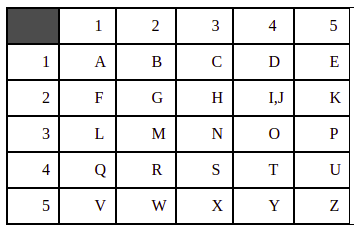
\includegraphics{polibi}
	\centering
	\caption{квадрат Полибия}
\end{figure}

Пары (i,j) передавались с помощью факелов. Например, для передачи буквы О нужно было взять 3 факела в правую руку и 4 – в левую.

Подобные шифровальные приспособления, с небольшими изменениями просуществовали до эпохи военных походов Юлия Цезаря. Положение меняется в эпоху расцвета Рима, который первоначально представлял собой лишь небольшую гражданскую общину, со временем он разросся, подчинив себе Италию, а затем всё Средиземноморье. Чтобы управлять наместниками в многочисленных провинциях, шифрованная связь для римских органов власти стала жизненно необходимой. Особую роль в сохранении тайны сыграл способ шифрования, предложенный Юлием Цезарем и изложенным им в «Записках о галльской войне» (1 век до Н.Э.) Вот что пишет о нём Гай Светоний «…существуют и его письма к Цицерону и письма к близким о домашних делах: в них, если нужно было сообщить что-то негласно, он пользовался тайнописью, то есть менял буквы так, чтобы из них не складывалось ни одного слова. Чтобы разобрать и прочитать их, нужно читать всякий раз четвёртую букву вместо первой, например, D вместо А и так далее». Таким образом, Цезарь заменял буквы в соответствии с подстановкой, нижняя строка которой представляет собой алфавит открытого текста, сдвинутый циклически на 3 буквы влево.\cite{senthil2013modern}

\subsection{Средневековые шифры}
%Шифры времен средневековья. Шифр Виженера. 

Шифровальный диск представлял собой пару соосных дисков разного диаметра. Больший из них – неподвижный, его окружность разделена на 24 равных сектора, в которые вписаны 20 букв латинского алфавита в их естественном порядке и 4 цифры. При этом из 24-х буквенного алфавита были удалены 4 буквы, без которых можно обойтись, подобно тому, как в русском языке обходятся без Ъ, Ё, Й. Меньший диск – подвижный, по его окружности, разбитой также на 24 сектора, были вписаны все буквы смешанного латинского алфавита.

\begin{figure}[H]
	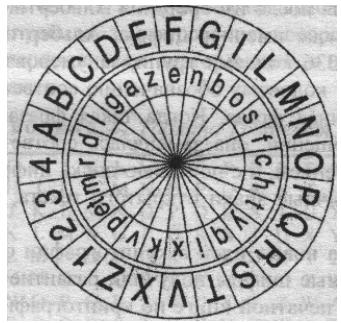
\includegraphics[scale=1.2]{alberti}
	\centering
	\caption{диск Альберти}
\end{figure}


Имея два таких прибора, корреспонденты догадывались о первой индексной букве на подвижном диске. При шифровании сообщения отправитель ставил индексную букву против любой буквы большого диска. Он информировал корреспондента о таком положении диска, записывая эту букву внешнего диска в качестве первой буквы шифртекста. Очередная буква открытого текста отыскивалась на неподвижном диске и стоящая против неё буква меньшего диска являлась результатом её зашифрования. После того как были зашифрованы несколько букв текста, положение индексной буквы изменялось, о чём также сообщалось корреспонденту.

Такой шифр имел две особенности, которые делают изобретение Альберти событием в истории криптографии. Во-первых, в отличие от шифров простой замены шифровальный диск использовал не один, а несколько алфавитов для зашифрования. Такие шифры получили название многоалфавитных. Во-вторых, шифровальный диск позволял использовать так называемые коды с перешифрованием, которые получили широкое распространение лишь в конце XIX в., то есть спустя четыре столетия после изобретения Альберти. Для этой цели на внешнем диске имелись цифры. Альберти составил код, состоящий из 336 кодовых групп, занумерованных от 11 до 4444. Каждому кодовому обозначению соответствовала некоторая законченная фраза. Когда такая фраза встречалась в открытом сообщении, она заменялась соответствующим кодовым обозначением, а с помощью диска цифры зашифровы­вались как обычные знаки открытого текста, превращаясь в буквы.

Богатым на новые идеи в криптографии оказался XVI в. Многоалфавитные шифры получили развитие в вышедшей в 1518 г. первой печатной книге по криптографии под названием "Полиграфия". Автором книги был один из самых знаме­нитых ученых того времени аббат Иоганнес Тритемий. В этой книге впервые в криптографии появляется квадратная таблица. Шифралфавиты записаны в строки таблицы один под дру­гим, причем каждый из них сдвинут на одну позицию влево по сравнению с предыдущим (см. табл. 2).

Тритемий предлагал использовать эту таблицу для многоалфавитного зашифрования самым простым из возможных способов: первая буква текста шифруется первым алфавитом, вторая буква — вторым и т. д. В этой таблице не было отдельного алфавита открытого текста, для этой цели служил алфавит первой строки. Таким образом, открытый текст, начинающийся со слов HUNC CAVETO VIRUM ..., приобретал вид HXPF GFBMCZ FUEIB ... .

Преимущество этого метода шифрования по сравнению с методом Альберти состоит в том, что с каждой буквой задействуется новый алфавит. Альберти менял алфавиты лишь по­сле трех или четырех слов. Поэтому его шифртекст состоял из отрезков, каждый из которых обладал закономерностями открытого текста, которые помогали вскрыть криптограмму. Побуквенное зашифрование не дает такого преимущества. Шифр Тритемия является также первым нетривиальным примером периодического шифра. Так называется многоалфавитный шифр, правило зашифрования которого состоит в использовании периодически повторяющейся последовательности простых замен.

\begin{figure}[H]
	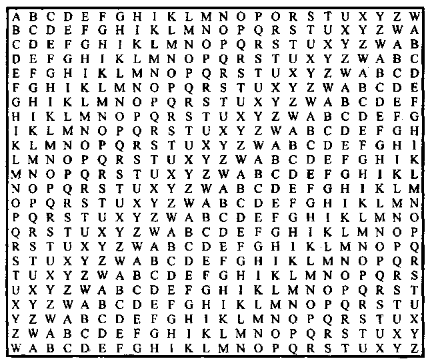
\includegraphics[scale=0.9]{trite}
	\centering
	\caption{таблица Тритемия}
\end{figure}



В 1553 г. Джованни Баттиста Белазо предложил использовать для многоалфавитного шифра буквенный, легко запо­минаемый ключ, который он назвал паролем. Паролем могло служить слово или фраза. Пароль периодически записывался над открытым текстом. Буква пароля, расположенная над буквой текста, указывала на алфавит таблицы, который исполь­зовался для зашифрования этой буквы. Например, это мог быть алфавит из таблицы Тритемия, первой буквой которого являлась буква пароля. Однако Белазо, как и Тритемий, использовал в качестве шифралфавитов обычные алфавиты.

Еще одно важное усовершенствование многоалфавитных систем, состоящее в идее использования в качестве ключа текста самого сообщения или же шифрованного текста, при­надлежит Джероламо Кардано и Блезу де Виженеру. Такой шифр был назван самоключом. В книге Виженера 'Трактат о шифрах" самоключ представлен следующим образом. В про­стейшем случае за основу бралась таблица Тритемия с добав­ленными к ней в качестве первой строки и первого столбца алфавитами в их естественном порядке. Позже такая таблица стала называться таблицей Виженера. Подчеркнем, что в общем случае таблица Виженера состоит из циклически сдви­гаемых алфавитов, причем первая строка может быть произ­вольным смешанным алфавитом (см. рис. \ref{tablvij}).

\begin{figure}[H]
	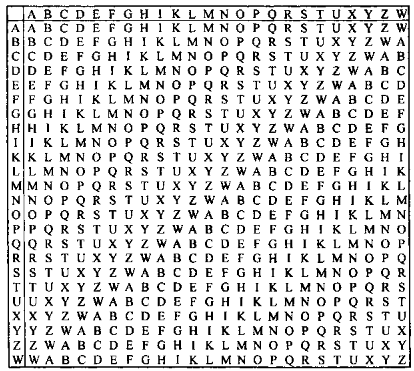
\includegraphics[scale=0.9]{vij}
	\centering
	\caption{таблица Вижинера}
	\label{tablvij}
\end{figure}


В истории криптографии XVII — XVIII в. называют эрой "черных кабинетов". В этот период во многих государствах Европы, в первую очередь во Франции, получили развитие дешифровальные подразделения, названные "черными кабинетами". Первый из них образован по инициативе кардинала Ришелье при дворе короля Людовика XIII. Его возглавил первый профессиональный криптограф Франции Антуан Россиньоль. Следует отметить, что некоторые оригинальные идеи, возникшие в криптографии в этот период, связаны с именем самого Ришелье, который использовал, например, для секретной переписки с королем оригинальный шифр перестановки с переменным ключом.

Много новых идей в криптографии принес XIX в. Изобретение в середине XIX в. телеграфа и других технических видов связи дало новый толчок развитию криптографии. Информация передавалась в виде токовых и бестоковых посылок, то есть представлялась в двоичном виде. Поэтому возникла проблема "рационального" представления информа ции, которая решалась с помощью кодов. Коды позволяли передать длинное слово или целую фразу двумя-тремя знаками. Появилась потребность в высокоскоростных способах шифрования и в корректирующих кодах, необходимых в связи с неизбежными ошибками при передаче сообщений \cite{omran2011cryptanalytic}.

Во второй половине XIX в. появился весьма устойчивый способ усложнения числовых кодов — гаммирование. Он заключался в перешифровании закодированного сообщения с помощью некоторого ключевого числа, которое и называлось гаммой. Шифрование с помощью гаммы состояло в сложении всех кодированных групп сообщения с одним и тем же ключевым числом. Эту операцию стали называть "наложением гаммы". Например, результатом наложения гаммы 6413 на кодированный текст 3425 7102 8139 являлась числовая последовательность 9838 3515 4552.


\subsection{Криптография первой мировой войны}
%Шифровальная машина Энигма. Работы Алана Тьюринга. Шифровальная техника СССР.
Первая мировая война оставила свой отпечаток на всех процессах, происходивших в человеческом обществе. Она не могла не сказаться и на развитии криптографии.

В период первой мировой войны в качестве полевых шифров широко использовались ручные шифры, в первую очередь шифры перестановки с различными усложнениями. Это были вертикальные перестановки, усложненные перекодировкой исходного алфавита, а также двойные вертикальные перестановки.

Первая мировая война явилась поворотным пунктом в истории криптографии: если до войны криптография представляла собой достаточно узкую область, то после войны она стала широким полем деятельности. Причина этого состояла в необычайном росте объема шифрпереписки, передаваемой по различным каналам связи. Криптоанализ стал важнейшим элементом разведки \cite{d2006sov}.

Прогресс этой области криптографии характеризовался и изменениями в самом криптоанализе. Эта наука переросла методы индивидуальной работы криптоаналитика над криптограммой. Системы секретной связи перестали быть настолько малочисленными и однородными, что один специалист мог овладеть всеми специализациями. Характер используемых шифров потребовал для их вскрытия скрупулезного анализа переписки, поиска ситуаций, благоприятствующих успешному криптоанализу, знания соответствующей обстановки. Кроме того, криптоанализ обогатился большим опытом использования в годы войны ошибок неопытных или ленивых шифровальщиков. Еще Ф. Бэкон писал, что "в результате неловкости и неискусности тех рук, через которые проходят величайшие секреты, эти секреты во многих случаях оказывались обеспеченными слабейшими шифрами". Этот печальный опыт привел к необходимости введения строгой дисциплины среди шифровальщиков.

Несмотря на указанные последствия, первая мировая война не породила никаких новых научных идей в криптографии. Наоборот, полностью исчерпали свои возможности ручное шифрование, с одной стороны, и техническая сторона криптоанализа, состоявшая в подсчете частот встречаемости знаков, с другой \cite{g2005n}.

\begin{figure}[H]
	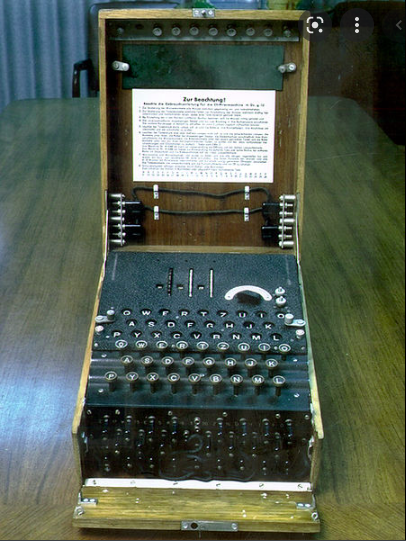
\includegraphics{enigma}
	\centering
	\caption{шифровальный аппарат Enigma \cite{hodges2014alan}}
\end{figure}



\subsection{Современной криптографии}
%Особенности современной криптографии. Теоретическая ненадежность современной криптографии.

В семидесятых годах произошло два события, серьезно повлиявших на дальнейшее развитие криптографии. Во-первых, был принят (и опубликован!) первый стандарт шифрования данных (DES), "легализовавший" принцип Керкгоффса в криптографии. Во-вторых, после работы американ­ских математиков У. Диффи и М. Хеллмана родилась "новая криптография"— криптография с открытым клю­чом. Оба этих события были рождены потребностями бурно развивающихся средств коммуникаций, в том числе локаль­ных и глобальных компьютерных сетей, для защиты которых потребовались легко доступные и достаточно надежные крип­тографические средства. Криптография стала широко востребоваться не только в военной, дипломатической, государст­венной сферах, но также в коммерческой, банковской и дру­гих сферах.

Вслед за идеей Диффи и Хеллмана, связанной с гипотетическим понятием однонаправленной (или односторонней) функции с секретом, появились "кандидат" на такую функ­цию и реально осуществленная шифрсистема RSA с откры­тым ключом. Такая система была предложена в 1978 г. Райвестом, Шамиром и Адлеманом. Парадоксальным казалось то, что в RSA для зашифрования и расшифрования используются разные ключи, причем ключ зашифрования может быть от­крытым, то есть всем известным. Вслед за RSA появился целый ряд других систем. В связи с несимметричным исполь­зованием ключей стал использоваться термин асимметричная шифрсистема, в то время как традиционные шифрсистемы стали называться симметричными.

Наряду с идеей открытого шифрования Диффи и Хеллман предложили идею открытого распределения ключей, позво­ляющую избавиться от защищенного канала связи при рас­сылке криптографических ключей. Их идея основывалась на сложности решения задачи дискретного логарифмировании, то есть задачи, являющейся обратной для задачи возведения в степень в конечном поле большого порядка \cite{bellare2005introduction}.

\begin{figure}[H]
	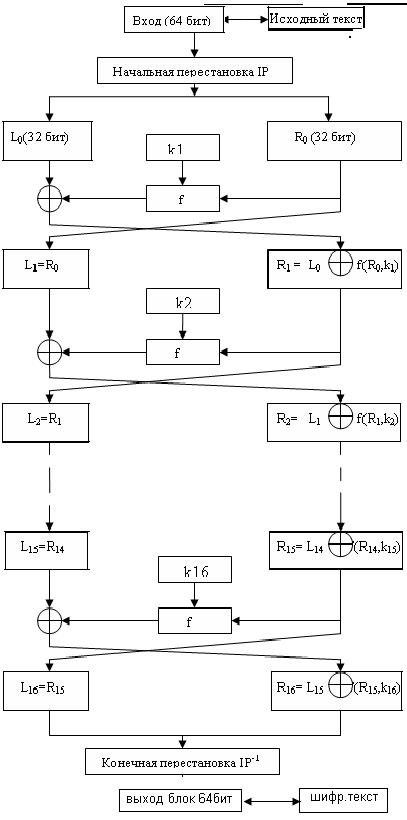
\includegraphics{des}
	\centering
	\caption{алгоритм шифрования DES}
\end{figure}


\section{Перспективы развития}
%Особенности квантовой криптографии. Её надежность.

Квантовая криптография — метод защиты коммуникаций, основанный на определенных явлениях квантовой физики \cite{ch1984quantum, lo2005decoy}. В отличие от традиционной криптографии, которая использует математические методы, чтобы обеспечить секретность информации, квантовая криптография сосредоточена на физике, рассматривая случаи, когда информация переносится с помощью объектов квантовой механики. Процесс отправки и приёма информации всегда выполняется физическими средствами, например при помощи электронов в электрическом токе, или фотонов в линиях волоконно-оптической связи. А подслушивание может рассматриваться, как измерение определённых параметров физических объектов — в нашем случае, переносчиков информации.

Технология квантовой криптографии опирается на принципиальную неопределённость поведения квантовой системы — невозможно одновременно получить координаты и импульс частицы, невозможно измерить один параметр фотона, не исказив другой. Это фундаментальное свойство природы в физике известно как принцип неопределённости Гейзенберга, сформулированный в 1927 г.

Используя квантовые явления, можно спроектировать и создать такую систему связи, которая всегда может обнаруживать подслушивание. Это обеспечивается тем, что попытка измерения взаимосвязанных параметров в квантовой системе вносит в неё нарушения, разрушая исходные сигналы, а значит, по уровню шума в канале легитимные пользователи могут распознать степень активности перехватчика.

\begin{figure}[H]
	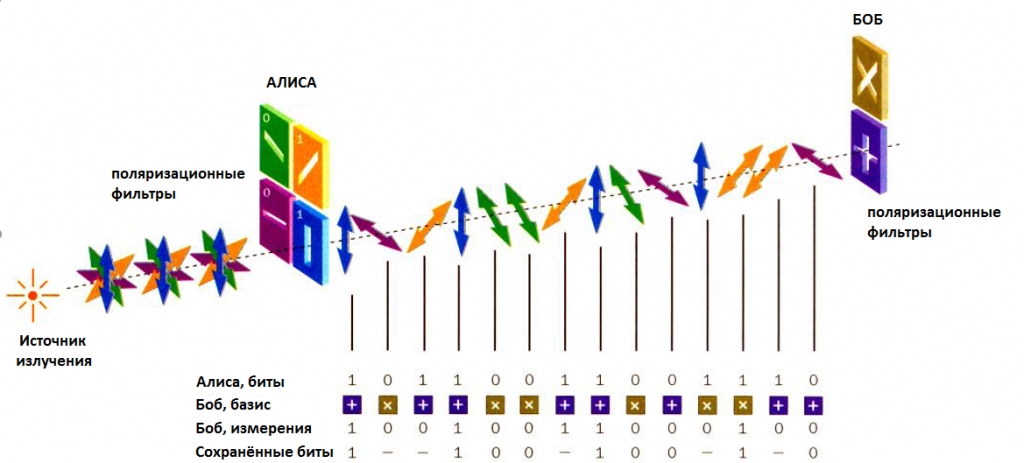
\includegraphics[scale=0.6]{BB84}
	\centering
	\caption{иллюстрация протокола BB84}
\end{figure}

\clearpage

\section*{Заключение}
%Общий вывод об истории криптографии, как науки и обзор дальнейших перспектив развития.

Появление в середине двадцатого столетия первых электронно-вычислительных машин кардинально изменило ситуацию в области шифрования (криптографии). С проникновением компьютеров в различные сферы жизни возникла принципиально новая отрасль - информационная индустрия.

Проблема обеспечения необходимого уровня защиты информации оказалась (и это предметно подтверждено как теоретическими исследованиями, так и опытом практического решения) весьма сложной, требующей для своего решения не просто осуществления некоторой совокупности научных, научно-технических и организационных мероприятий и применения специфических средств и методов, а создания целостной системы организационных мероприятий и применения специфических средств и методов по защите информации.

Объем циркулирующей в обществе информации стабильно возрастает. Популярность всемирной сети Интренет в последние годы способствует удваиванию информации каждый год. Фактически, на пороге нового тысячелетия человечество создало информационную цивилизацию, в которой от успешной работы средств обработки информации зависит благополучие и даже выживание человечества в его нынешнем качестве. Произошедшие за этот период изменения можно охарактеризовать следующим образом: объемы обрабатываемой информации возросли за полвека на несколько порядков; доступ к определенным данным позволяет контролировать значительные материальные и финансовые ценности; информация приобрела стоимость, которую даже можно подсчитать; характер обрабатываемых данных стал чрезвычайно многообразным и более не сводится к исключительно текстовым данным; информация полностью "обезличилась", т.е. особенности ее материального представления потеряли свое значение - сравните письмо прошлого века и современное послание по электронной почте; характер информационных взаимодействий чрезвычайно усложнился, и наряду с классической задачей защиты передаваемых текстовых сообщений от несанкционированного прочтения и искажения возникли новые задачи сферы защиты информации, ранее стоявшие и решавшиеся в рамках используемых "бумажных" технологий - например, подпись под электронным документом и вручение электронного документа "под расписку"; субъектами информационных процессов теперь являются не только люди, но и созданные ими автоматические системы, действующие по заложенной в них программе; вычислительные "способности" современных компьютеров подняли на совершенно новый уровень как возможности по реализации шифров, ранее немыслимых из-за своей высокой сложности, так и возможности аналитиков по их взлому.

\clearpage

\bibliography{refs}

\clearpage
\pagenumbering{gobble}
\section*{Отзыв научного руководителя на тему реферата}
Я, Черкесова Лариса Владимировна, научный руководитель аспиранта первого года обучения Галова Кирилла Алексеевича подтверждаю, что данная тема соответствует специальности 09.06.01 «Информатика и вычислительная техника» и направлению исследований аспиранта.
\bigskip

\rightline{проф. каф. «КБИС», д.ф.-м.н. \hspace{0.5cm} \underline{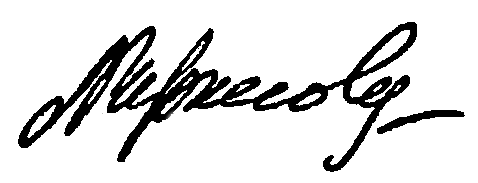
\includegraphics[width=3cm]{cherlv-podpis}} \hspace{0.5cm} Черкесова Л. В}

\end{document}